\section{Durchführung}
\label{sec:Durchführung}
Zunächst soll die Zeitabhängigkeit der Amplitude des gedämpften Schwingkreises auf
dem Oszilloskop sichtbar gemacht und daraus der Dämpfungsfaktor bestimmt werden.
Dafür wird die Schaltung aus \ref{fig:aufbau_1} benutzt. Im Gegensatz zur Schaltung in der Abbildung
wird jedoch Rechteckspannung statt einer Nadelimpulsspannung verwendet. In diesem
Versuch wird der geringe der beiden Widerstände benutzt.  Das Bild wird so eingestellt,
dass man einen Amplitudenverlauf möglichst genau erkennen kann. Das entstandene Bild
wird gespeichert. Daraufhin wird die Einhüllende eingezeichnet und es werden Werte
von dieser abgelesen.
\begin{figure}
  \centering
  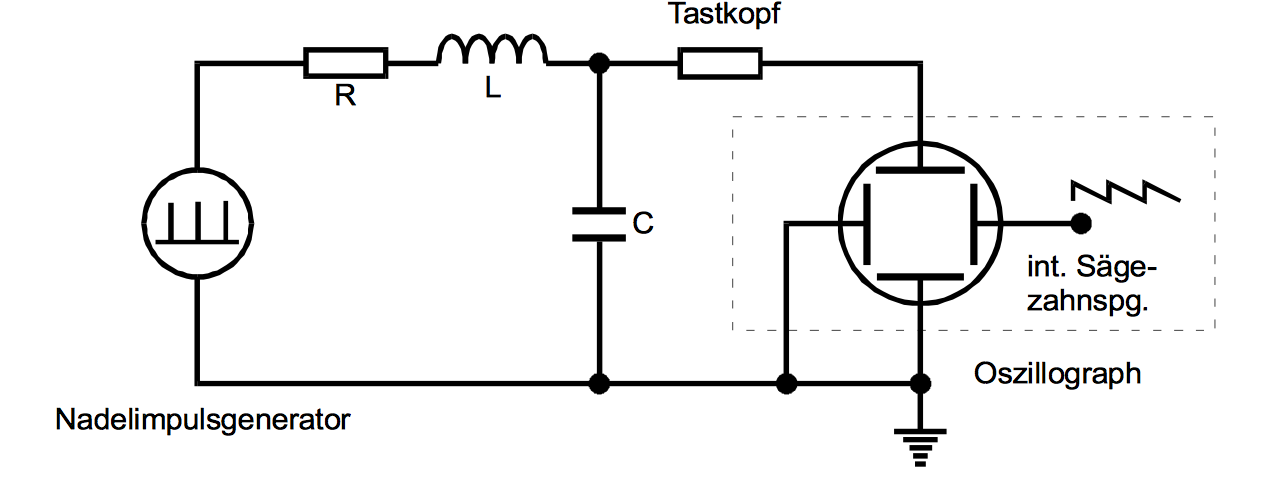
\includegraphics[width=300pt]{data/aufbau_1.png}
  \caption{Schaltung zur Bestimmtung der Zeitabhängigkeit der Amplitude der gedämpften
  Schwingung durch Beobachtung und Auswertung der Kondensatorspannung \cite{Versuchsanleitung1}}
  \label{fig:aufbau_1}
\end{figure}


Daraufhin soll der Widerstand ermittelt werden, bei dem der aperiodische Grenzfall
vorliegt. Dafür wird die Schaltung aus \ref{fig:aufbau_2} verwendet. Der Widerstand ist hierbei variabel
und wird zunächst auf sein Maximum geregelt. Nun wird der Widerstand so lange reduziert,
bis sich auf dem Oszilloskop eine Überschwingung der Amplitude erkennen lässt. Nun wird
der Widerstand wieder erhöht, bis gerade keine Überschwingung mehr erkennbar ist. Nun
wird der Wert für den Widerstand abgelesen.
\begin{figure}
  \centering
  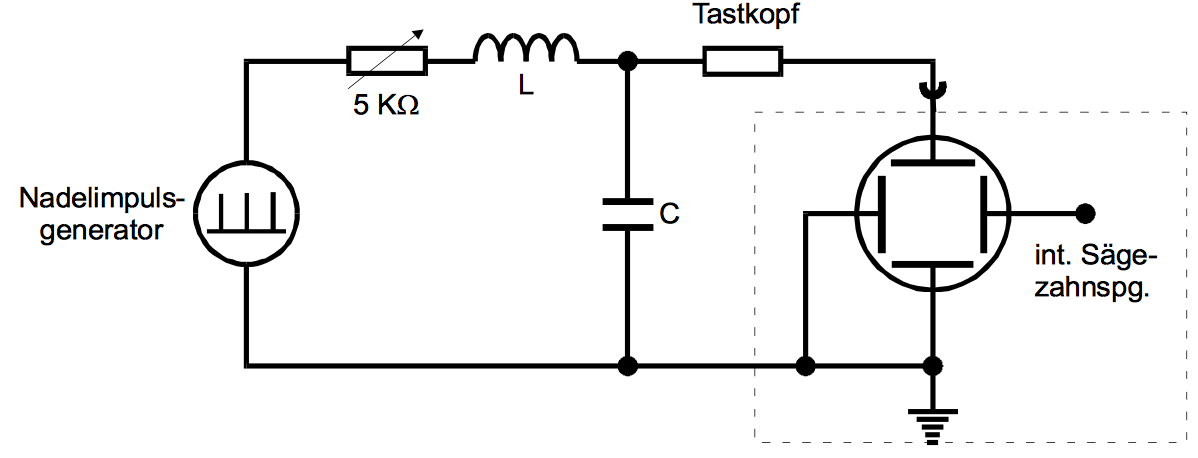
\includegraphics[width=300pt]{data/aufbau_2.png}
  \caption{Schaltung zur Bestimmtung des Widerstandes, bei dem sich der aperiodische
  Grenzfall einstellt \cite{Versuchsanleitung1}}
  \label{fig:aufbau_2}
\end{figure}


Im Anschluss daran soll die Spannung $\U_{\text{C}}$ am Kondensator in Abhängigkeit
von der anregenden Frequenz $f$ gemessen werden, wobei an den Schwingkreis eine
sinusförmige Spannung angelegt wird. Dafür wird die Schaltung aus \ref{fig:aufbau_3} verwendet,
jedoch wird hier zur Spannungsmessung ein Oszilloskop statt eines Millivoltmeters
verwendet. Nun wird über Frequenzen in verschiedenen Größenordnungen hinweg die
Spannung $\U_{\text{C}}$  am Kondensator gemessen. In Bereichen mit großen Änderungen
 werden dabei mehr Werte aufgenommen als in Bereichen mit wenig Änderungen.
Da der Tastkopf des Oszilloskops selbst ebenfalls eine Frequenzabhängigkeit besitzt,
wird daraufhin die erzeugte Spannung für die zuvor gewählten Frequenzen erneut mit
dem Tastkopf gemessen.
\begin{figure}
  \centering
  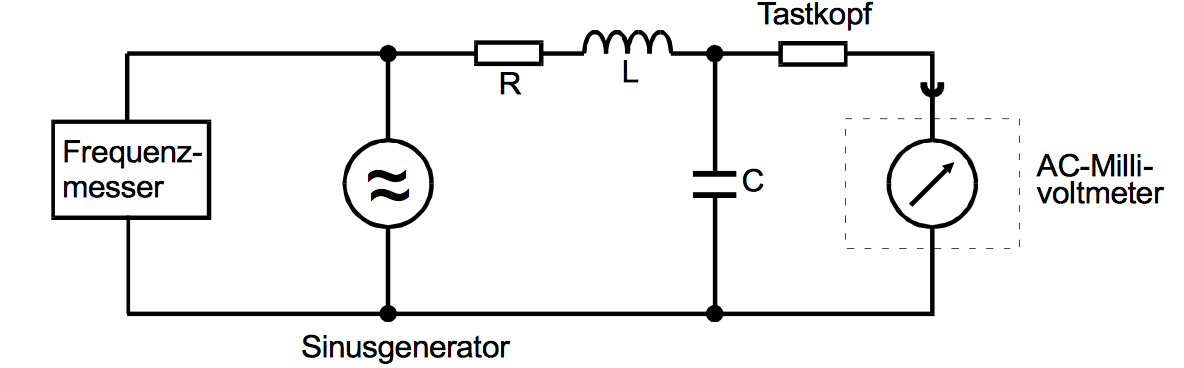
\includegraphics[width=300pt]{data/aufbau_3.png}
  \caption{Schaltung zur Bestimmtung der Abhängigkeit der Spannung am Kondensator
  in Abhängigkeit von der an den RLC-Kreis angelegten Frequenz\cite{Versuchsanleitung1}}
  \label{fig:aufbau_3}
\end{figure}


Zur Messung der Phasenverschiebung $\phi$ der Ausgangsspannung $U_{\text{G}}$ und
der Spannung $\U_{\text{C}}$ am Kondensator wird die Schaltung aus \ref{fig:aufbau_4} verwendet.
Beide Spannungen werden auf dem Oszilloskop dargestellt und gemäß \ref{fig:phasenverschiebung} wird der
zeitliche Unterschied der Nulldurchgänge der beiden Spannungen für Frequenzen
über mehrere Größenordnungen hinweg gemessen.
\begin{figure}
  \centering
  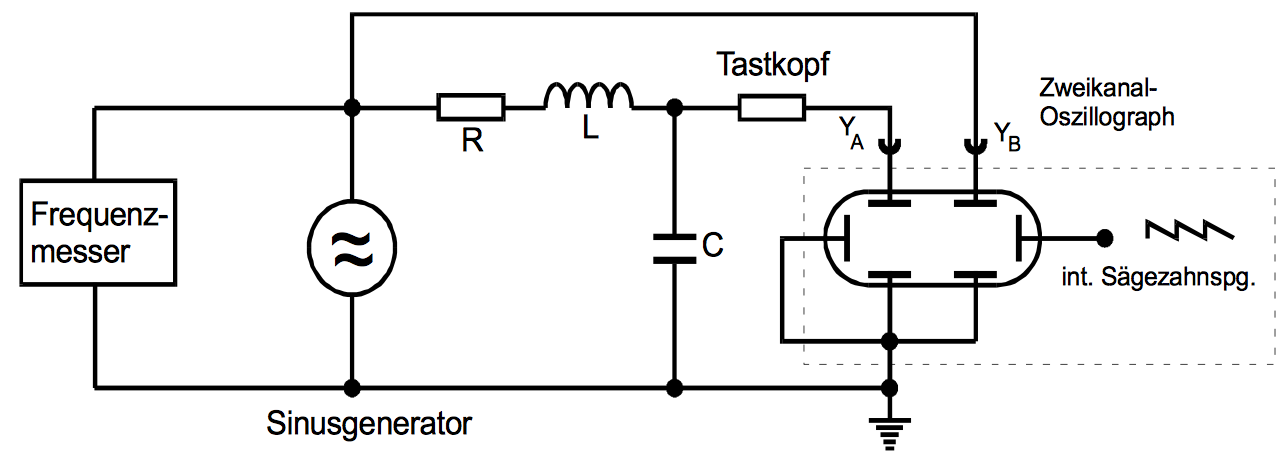
\includegraphics[width=300pt]{data/aufbau_4.png}
  \caption{Schaltung zur Bestimmtung der Abhängigkeit der Phasenverschiebung der
  Generatorspannung und der Spannung am Kondensator in Abhängigkeit von der
  an den RLC-Kreis angelegten Frequenz \cite{Versuchsanleitung1}}
  \label{fig:aufbau_4}
\end{figure}
\begin{figure}
  \centering
  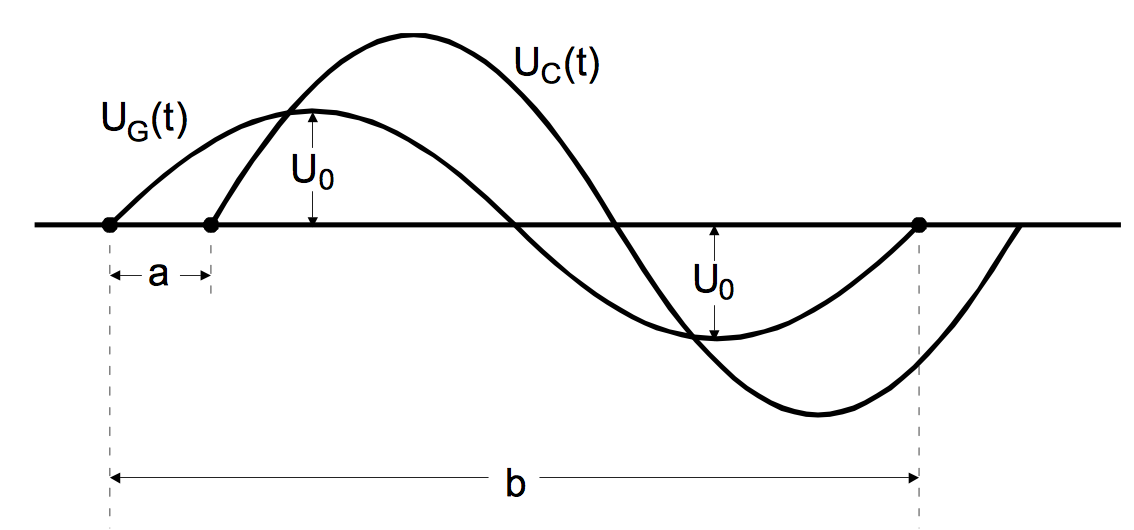
\includegraphics[width=300pt]{data/phasenverschiebung.png}
  \caption{Skizze zur Bestimmung der Phasenverschiebung \cite{Versuchsanleitung2}}
  \label{fig:phasenverschiebung}
\end{figure}
